% Created with jtex v.1.0.20
%%%%%%%%%%%%%%%%%%%%%%%%%%%%%%%%%%%%%%%%%%%%%%%%%%%%%%%%%%%%
%%% LaPreprint: PREPRINT TEMPLATE
%%%%%%%%%%%%%%%%%%%%%%%%%%%%%%%%%%%%%%%%%%%%%%%%%%%%%%%%%%%%

% Here I could talk about what one should do in this document.
% Instead I'll refer you to the explore on your own and check the Github Repo. :-)
% Line spacing is 1.2 by default (can't be smaller).

%%%%%%%%%%%%%%%%%%%%%%%%%%%%%%%%%%%%%%%%%%%%%%%%%%%%%%%%%%%%
%%% PREAMBLE
%%%%%%%%%%%%%%%%%%%%%%%%%%%%%%%%%%%%%%%%%%%%%%%%%%%%%%%%%%%%

% Declare document class
\documentclass[9pt,Preprint]{lapreprint}
% Choose between "biorxiv", "medrxiv", "arxiv" and "chemrxiv". Otherwise defaults "Preprint".
% Choose between "blue" and "red" colour scheme. Defaults to "blue".
% Use the "onehalfspacing" option for 1.5 line spacing.
% Use the "doublespacing" option for 2.0 line spacing.
% Use the "lineno" option for line numbers.
% Use the "endfloat" option to place floats after the bibliography.
% Use the "secnum" option to have include numbers.

% Import packages
% \usepackage{lipsum}     % Required to insert dummy text
\usepackage[version=4]{mhchem} % For chemical notation
\usepackage{siunitx}    % For SI units
\usepackage{pdflscape}  % For putting pages in landscape mode
\usepackage{rotating}   % For rotating specific elements
\usepackage{textgreek}  % Greek symbols
\usepackage{gensymb}    % Symbols
\usepackage[misc]{ifsym} % For the \Letter symbol
\usepackage{orcidlink}  % For the \orcidlink
\usepackage{listings}   % For inserting code chunks
\usepackage{colortbl}   % For Knitr table colouring
\usepackage{tabularx}   % For making Knitr tables compatible
\usepackage{longtable}  % For multi-page tables
\usepackage{subcaption}
\usepackage{multirow}
\usepackage{snotez}     % For sidenote environments. enotez for endnotes
\usepackage{csquotes}   % For language-based quote rules (helps BiBLaTeX)



% Make declarations
\DeclareSIUnit\Molar{M}

% Please note that these options may affect formatting.

%%%%%%%%%%%%%%%%%%%%%%%%%%%%%%%%%%%%%%%%%%%%%%%%%%%%%%%%%%%%
%%% BIBLIOGRAPHY
%%%%%%%%%%%%%%%%%%%%%%%%%%%%%%%%%%%%%%%%%%%%%%%%%%%%%%%%%%%%
\usepackage[			% use biblatex for bibliography
	backend=biber,      % use biber or bibtex backend
    style=authoryear,   % choose style
	natbib=true,		% allow natbib commands
	hyperref=true,	    % activate hyperref support
	alldates=year,      % only show year (not month)
]{biblatex}

% Just avoiding some rogue fields that cause issues with certain styles
\AtEveryBibitem{
    \clearfield{urlyear}
    \clearfield{urlmonth}
    \clearlist{language}
}

% Update to your bibliography file
\addbibresource{main.bib}


%%%%%%%%%%%%%%%%%%%%%%%%%%%%%%%%%%%%%%%%%%%%%%%%%%%%%%%%%%%%
%%% ARTICLE SETUP
%%%%%%%%%%%%%%%%%%%%%%%%%%%%%%%%%%%%%%%%%%%%%%%%%%%%%%%%%%%%

% Paper title
\title{CT scan reconstruction using machine learning}

% Authors - you can use \orcidlink{} and \authfn{} - see contribution note
\author[]{Luuk Froling}

% Affiliations

% Other metadata. Feel free to add your own
\metadata[]{Keywords}{Finite volume; Direct current; Resistivity; DC equations}


% Surname of the lead author(s) for the running footer
\leadauthor{Luuk Froling}
\shorttitle{Written by Luuk Fröling}

%%%%%%%%%%%%%%%%%%%%%%%%%%%%%%%%%%%%%%%%%%%%%%%%%%%%%%%%%%%%
%%% ARTICLE START
%%%%%%%%%%%%%%%%%%%%%%%%%%%%%%%%%%%%%%%%%%%%%%%%%%%%%%%%%%%%

\begin{document}
\maketitle


\textbf{Author:} Luuk Fröling

\section{abstract}

This will be the abstract

\section{Introduction}

This will be the introduction

\section{Theory}

\subsection{Basics CT scans}

A CT scan is an imaging technique which uses x-rays sto create cross-sectional images of the body. A CT scan machine consists of a source and a detector placed at a distance from eachother. During the imaging procedure, both the source and the detector will rotate around the object to be imaged. The source will emit x-rays which will partially travel through the object towards the detector. The detector will measure the spectrum of transmitted photons on the other side of the object to be imaged. The spectrum is shaped by how much of the x-rays are being absorbed or scattered by the body, which can be described as the number of detected photons $\hat{y}_i$, generally given as

\begin{equation}
\label{first }
\hat{y}_i  = N_0 \cdot \exp\left(-\int \mu(x, E) \, dx\right)
\end{equation}

where $N_0$ is the number of the x-rays entering the body, the subscript i denotes the location along the detector and the integral in the exponent represents the cumulative attenuation $\mu(x, E)$ of the x-ray beam along it's path x, where the linear attenuation coefficient $\mu(x, E)$ changes throughout the body \parencite{kamalian2016ct_principles}. When measureing $\hat{y}_i$ for a set of angles around the object to be imaged, a sinogram can be constructed by plotting $\hat{y}_i$ aginst the angle.

\begin{figure}[!htbp]
\centering
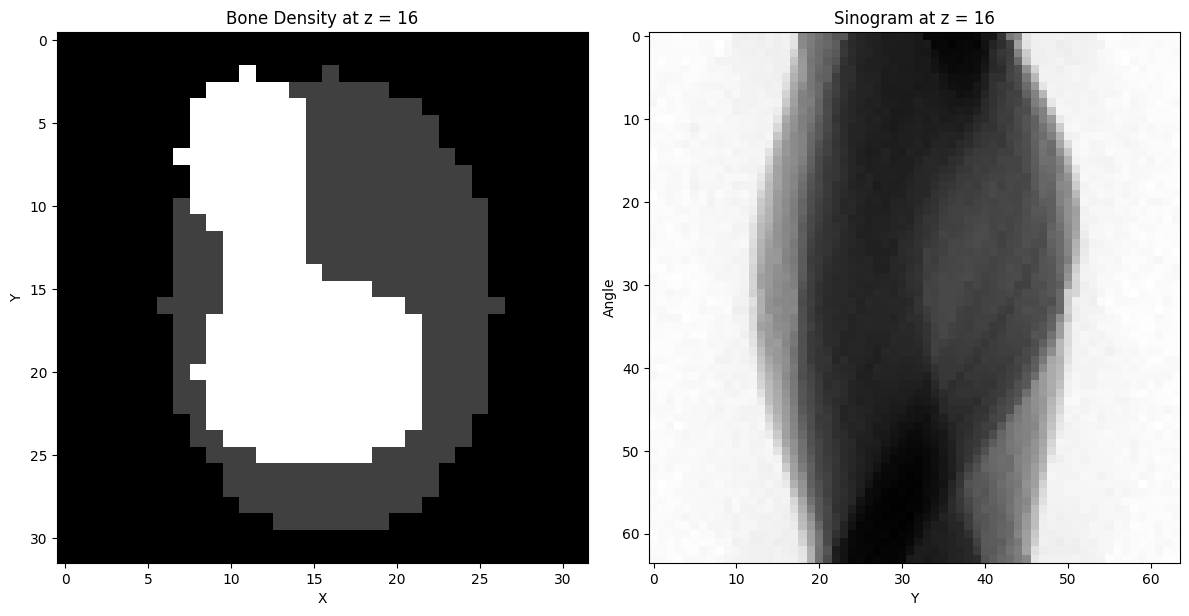
\includegraphics[width=0.7\linewidth]{files/b976b4c5294674aa189b37fdcfeb40f7.png}
\caption[]{\textit{left:} a 2D slice of the phantom the colour gradient representing bone density. \textit{right} corresponding sinogram with 64 projection angles and a detector size in the y-direction of 64 pixels - say what energy}
\label{phantomSinogram}
\end{figure}

Both a phantom and a corresponding sinogram can be seen in Figure~\ref{phantomSinogram}. Here the phantom shows the simulated bone density of an object, with lighter coloured areas having a higher bone density. On the right is the corresponding sinogram which consists of 64 measurements of $\hat{y}_i$ at different angles.

\subsection{Cone beam CT scan}

The sinogram in figure Figure~\ref{phantomSinogram} is true for a 1D detector, where we only measure along the Z-axis of the phantom. A cone beam CT scan uses a source which emits in a cone like shape and a 2D detector to measure the projections.

\begin{figure}[!htbp]
\centering
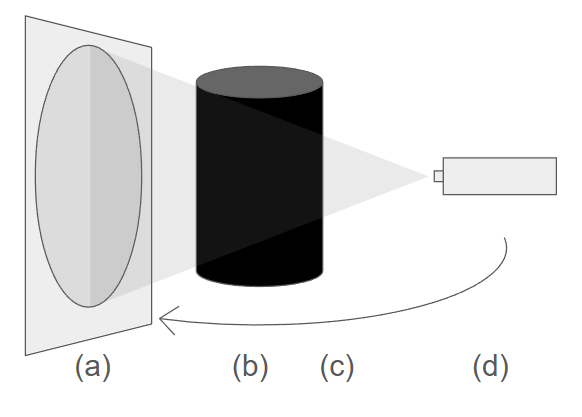
\includegraphics[width=0.5\linewidth]{files/cone_beam_ct-cf60e2b0345375bb14b01c570192d07f.png}
\caption[]{A schematic drawing of a cone beam CT scan procedure with (a) the detector measuring the projections in 2D, (b) the phantom, (c) the direction of rotation for both detector and the source and (d) the x-ray source.}
\label{cone_beam}
\end{figure}

For data reconstruction, a more complex backprojection algorithm needs to be used as we introduce the angle between the incomming x-rays onto the detector and the detector itself as a variable.

\subsection{Detector types}

Modern CT scan machines currently use an energy integrating detector (EID) \parencite{marth2023photon}. An EID measures the intensity of the incomming x-rays by a two-step process: scintillation followed by photodetection.

There are 2 main issues with these detectors we will focus on:

\begin{itemize}
\item The contrast between different soft tissues is often insufficient
\item images are not tissue-type specific
\end{itemize}

These detectors measure by the energy-integrated signal of photons \parencite{taguchi2013photon} which loses all energy dependent information.

\begin{figure}[!htbp]
\centering
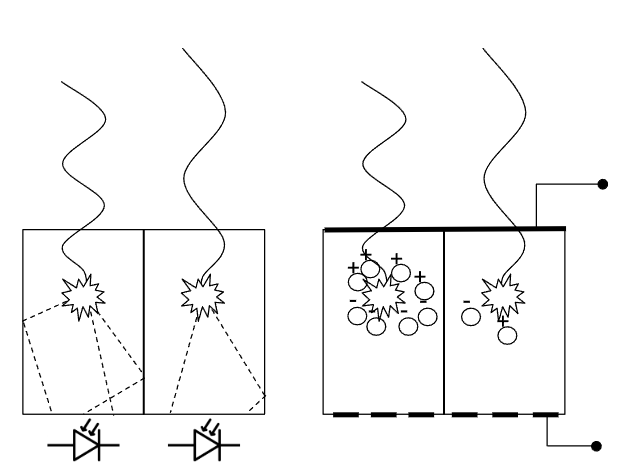
\includegraphics[width=0.7\linewidth]{files/detectorTypes-8bd48a755bc03e91c0cd2be80c4a4001.png}
\caption[]{\textit{left:} energy integrating detector. \textit{right:} photon counting detector}
\label{detectors}
\end{figure}

To be able to simulate a body in a CT scan, material decompositon \parencite{mechlem2018joint} can be used. The linear attenuation coëfficient at location x will be

\subsection{Material decomposition}
\begin{equation}
\label{muE}
\mu(E) = \sum_{b=1}^{B} A_b f_b(E)
\end{equation}
where $A_b$ is the line integral of material b and $f^b(E)$ describes the attenuation coefficient of the basis material b. Combining the equation (\ref{first}) and (\ref{muE}) gives an expression for the photon count at the detector:

something relating I to y\_i
\begin{equation}
\hat{y}_i = \int_0^{\infty} \phi_{\text{eff},i}(E) \exp\left( - \sum_{b=1}^{B} A_b^i f_b(E) \right) \, dE
\end{equation}

\begin{figure}[!htbp]
\centering
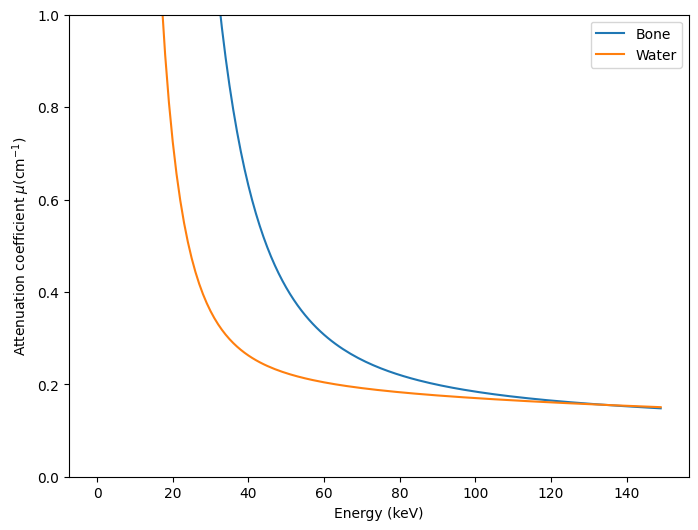
\includegraphics[width=0.7\linewidth]{files/64ccdbd7840b97b269bc4a429597ebd6.png}
\caption*{The attenuation coefficient of bone (blue) and water (orange) plotted against the energy of the incomming photons.}
\end{figure}

During a CT-scan $\hat{y}_i$ is measured for a set of angles. Each measurement results in a 1D array for a 2D slice.

Recent breakthroughs in photon counting detectors make use of equation (\ref{muE}), where the linear attentuation coefficient depends on the energy level. The photon counting detectors (pcd) allow the classification of measured photons into energy bins \parencite{pcd2022}.

\subsection{Projection algorithms}

\begin{itemize}
\item brief overview backprojection  \parencite{zeng2001image}


\item list issues


\item brief overview itterative approach (with references to Mechlem)


\item positives


\item negatives
\end{itemize}

part of abstract: ``g. They require a specific
reconstruction process, consisting of two steps: material decomposition and tomographic
reconstruction. Image-based methods perform reconstruction, then decomposition, while
projection-based methods perform decomposition first, and then reconstruction. As an alternative,
`one-step inversion' methods have been proposed, which perform decomposition and reconstruction
simultaneously. Unfortunately, one-step methods are typically slower than their two-step
counterparts, and in most CT applications, reconstruction time is critical. This paper therefore
proposes to compare the convergence speeds of five one-step algorithms.'' \parencite{mory2018comparison}

itterative unet \parencite{ge2023mb}

\subsection{machine learning - neural networks}

Neural networks are a subset of machine learning and play a crucial role in deep learning algorithms. In the basis, neural networks consist of a number of nodes. A set of nodes are combined into layers where all layers are connected by weights. Starting from the input layer, each input node corresponding with a number is connected to every node in the first layer with a weight. to calculate the value of a node in the next layer, all node from the previous layer are multiplied by the weight connecting them. Stacking layers after eachother creates a neural network.

Neural networks learn by backpropagation. Backpropagation looks at the error between the output of the network and the desired output. This error is generally backpropogated through the network by looking at how each weight needs to change to minimise the error.

\subsection{machine learning - CNN}

A convolutional neural network can be used to more accuratly extract features from images for processing. A convolutional neural network consist of a kernel and an amount of channels. The kernel has an equal number of dimensions as the input data however smaller which consists of weights. The kernel will move across the input data performing element wise multiplication with the part of the input they cover, extracting information like edges, textures and shapes \parencite{yamashita2018convolutional}.

\begin{figure}[!htbp]
\centering
\begin{verbatim}
Text(0, 0.5, 'Y')
\end{verbatim}

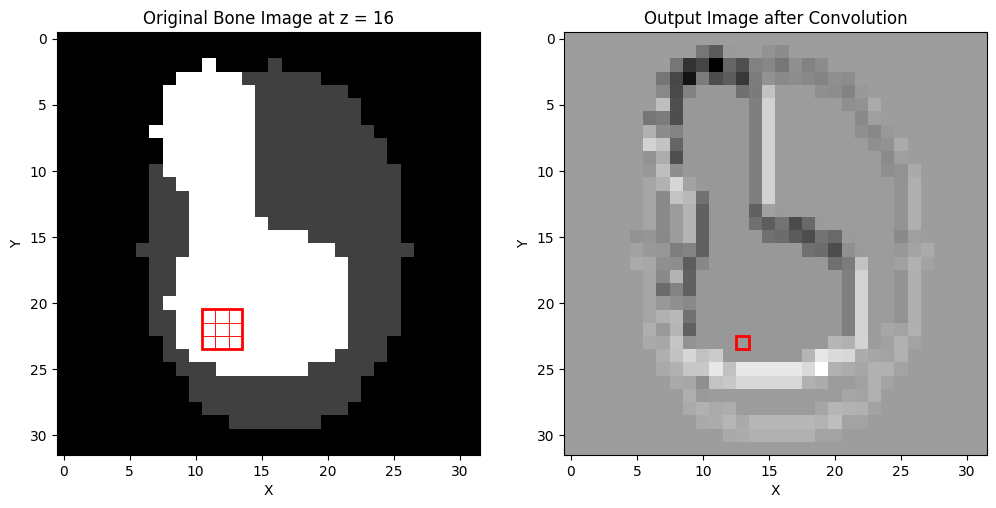
\includegraphics[width=0.7\linewidth]{files/53dfddea48d84244f37a3a2bae253fa3.png}
\caption*{\textit{left :} original phantom with a 2D 3x3 randomly initialised kernel drawn on top. each individual square represents a pixel, with the outer square representing the kernel. \textit{right :} phantom after 2D convolution layer has been applied.}
\end{figure}

\begin{itemize}
\item UNet github\parencite{ronneberger2015u}
\end{itemize}

\subsection{Machine learning - Attention}

An attention mechanism is a technique used in machine learning which is used to allow machine learning models to attend to the most relevant parts of the input data \parencite{vaswani2017attention}.

\begin{figure}[!htbp]
\centering
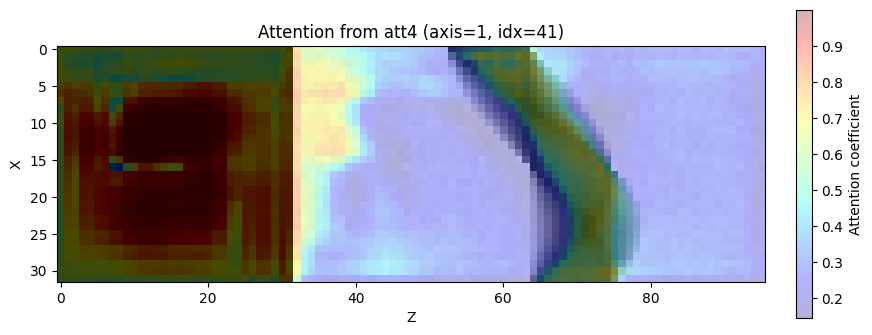
\includegraphics[width=0.7\linewidth]{files/61e001e87d8f0264596b2282806f90e4.png}
\caption*{: label : attention\_network
An attention map showing how an attention mechanism can be used to have the model focus more on important features, which in this case is the sinogram.}
\end{figure}

\begin{itemize}
\item attention map?
\item How we want to map the sinogram to the image, which is non-local \parencite{vaswani2017attention}
\end{itemize}

\subsection{Machine learning - UNet with attention}

How multiple convolutions and attention networks can be combine to edit images

\section{Method}

\subsection{acquiring data}

A machine learning model will be trained to convert an image from sinogram space to image space. This will be done according to the steps taken in an iterative approach \parencite{mechlem2018joint} and the model will be trained on the intermediate steps calculated. To be able to train the model we need 2 sorts of data:

\begin{itemize}
\item projection matrix
\item images during reconstruction
The projection matrix will have the dimensions of the number of projections x y pixels detector x z pixels detector. The images during reconstruction refer to the intermediate images between each iteration of the iterative algorithm. As both parts of the data have a 3D format, the images will be padded with 0's to match the y-dimension of the projection matrix. The image and the projection are appended in the z-direction.
\end{itemize}

\begin{figure}[!htbp]
\centering
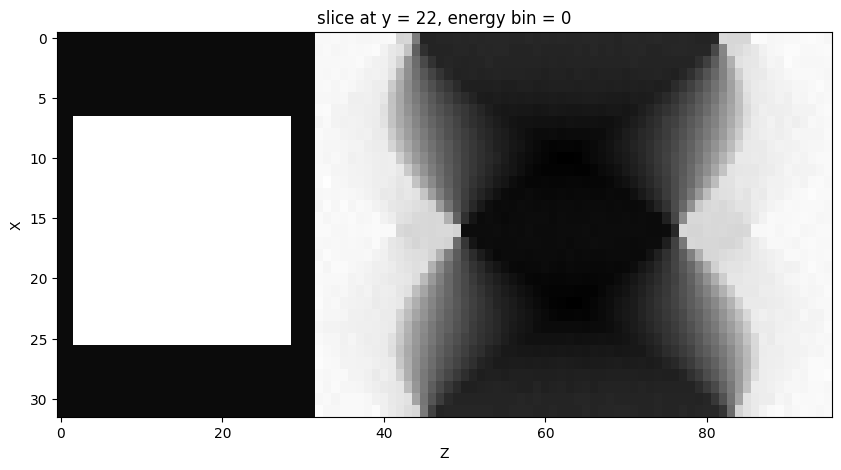
\includegraphics[width=0.7\linewidth]{files/536cee391b3c3bc26ab19b0a44ac3068.png}
\caption[]{\textit{left:} example of input data, where on the left we see a square which is a cross section of a 3D cylinder. On the right corresponding sinogram. Axes don't line up!}
\label{input}
\end{figure}

\begin{itemize}
\item how many mechlem runs
\item how many iterations
\item stride of the input images
\end{itemize}

\subsection{Attention based UNet}

UNet has already been used to segmented, based on github

\begin{figure}[!htbp]
\centering
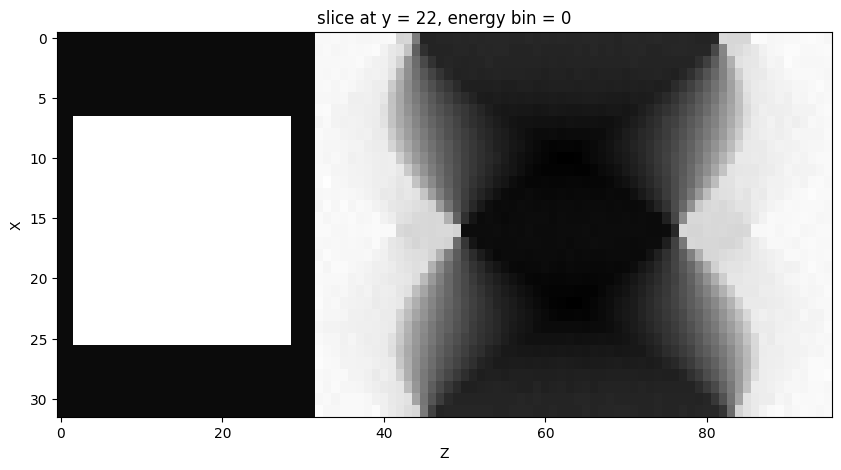
\includegraphics[width=0.7\linewidth]{files/536cee391b3c3bc26ab19b0a44ac3068.png}
\caption[]{\textit{left:} example of input data, where on the left we see a square which is a cross section of a 3D cylinder. On the right corresponding sinogram. Axes don't line up!}
\label{input}
\end{figure}

what network has finally been constructed etc

\subsection{curriculum learning}

Collected data \{number from notebook\}

\begin{figure}[!htbp]
\centering
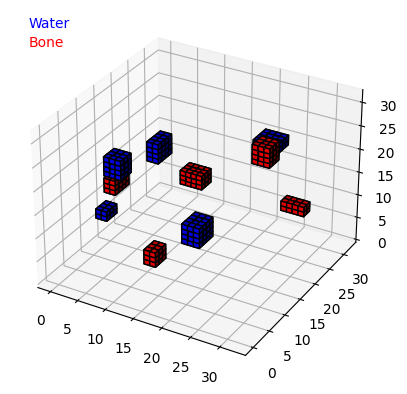
\includegraphics[width=0.7\linewidth]{files/641b1a53d2694f4e97f89c13e2f487a6.png}
\caption[]{\textit{left:} Single data set used for curriculum learning.}
\label{c3d}
\end{figure}

\subsection{Training on phantoms}

Collected \{number from notebook\} sets of training data which will be implemented with the following parameters:

\section{results}

\subsection{plot about speedup (time vs pixel size)}

either 2D or 3D

\subsection{plot about results for 32x32 simple phantom}

\subsection{plot harder phantom (3 features or more)}

\section{Discussion}

\subsection{non-machine learning speedup}

pytorch is highly optimized, mechlem is not

\subsection{pixel size and number of projections necessary}

There will not be a linear relationship between the amount of projections necessary and the amount of pixels in the image. will this have an impact?

\printbibliography

% DON'T EDIT. If "endfloat" option is enabled all floats appear before appendices
\if@endfloat\clearpage\processdelayedfloats\clearpage\fi


%%%%%%%%%%%%%%%%%%%%%%%%%%%%%%%%%%%%%%%%%%%%%%%%%%%%%%%%%%%%
%%% SUPPLEMENTARY MATERIAL / APPENDICES
%%%%%%%%%%%%%%%%%%%%%%%%%%%%%%%%%%%%%%%%%%%%%%%%%%%%%%%%%%%%
%% Sadly, we can't use floats in the appendix boxes. So they don't "float", but use \captionof{figure}{...} and \captionof{table}{...} to get them properly caption.

%%%%%%%%%%%%%%%%%%%%%%%%%%%%%%%%%%%%%%%%%%%%%%%%%%%%%%%%%%%%
%%% ARTICLE END
%%%%%%%%%%%%%%%%%%%%%%%%%%%%%%%%%%%%%%%%%%%%%%%%%%%%%%%%%%%%

\end{document}
